

\chapter{Petri nets overview}
%\addcontentsline{toc}{chapter}{Brief introduction to contPN}
%\markboth{Brief introduction to contPN}{Brief introduction to contPN}

Hybrid Petri nets~\cite{BODavid10,ARBaMeGi00} represent a powerful modeling formalism
that allows the integration of both continuous and discrete dynamics in a single net model. This
section defines the class of hybrid nets supported by $SimHPN$. In the following, the reader
is assumed to be familiar with Petri nets (PNs) (see \cite{ARMura89,BODHPSV93}
for a gentle introduction).

\section{Untimed Hybrid Petri net  systems}
\label{s:untimedHPN}

\begin{defn}
\label{d:uhpn}
A \emph{Hybrid Petri Net (HPN) system} is a pair $\sys$, where: $\N = \langle
P,T,\Pre,\Post\rangle$ is a \emph{net structure}, with set of places
$P$, set of transitions $T$, pre and post incidence matrices
$\Pre, \Post \in \rea^{|P|\times |T|}_{\geq 0}$, and $\b{m}_0\in \rea^{|P|}_{\geq 0}$ is the
\emph{initial marking}.
\end{defn}

% Definition of structural elements
The token load of the place $p_i$ at marking $\b{m}$ is denoted by
$m_i$ and the \emph{preset} and \emph{postset} of a node $X \in P \cup
T$ are denoted by $\preset{X}$ and $\postset{X}$, respectively. For
a given incidence matrix, e.g., $\Pre$, $\Pre(p_i,t_j)$ denotes the element of
$\Pre$ in row $i$ and column $j$.

\begin{figure*}
\centering
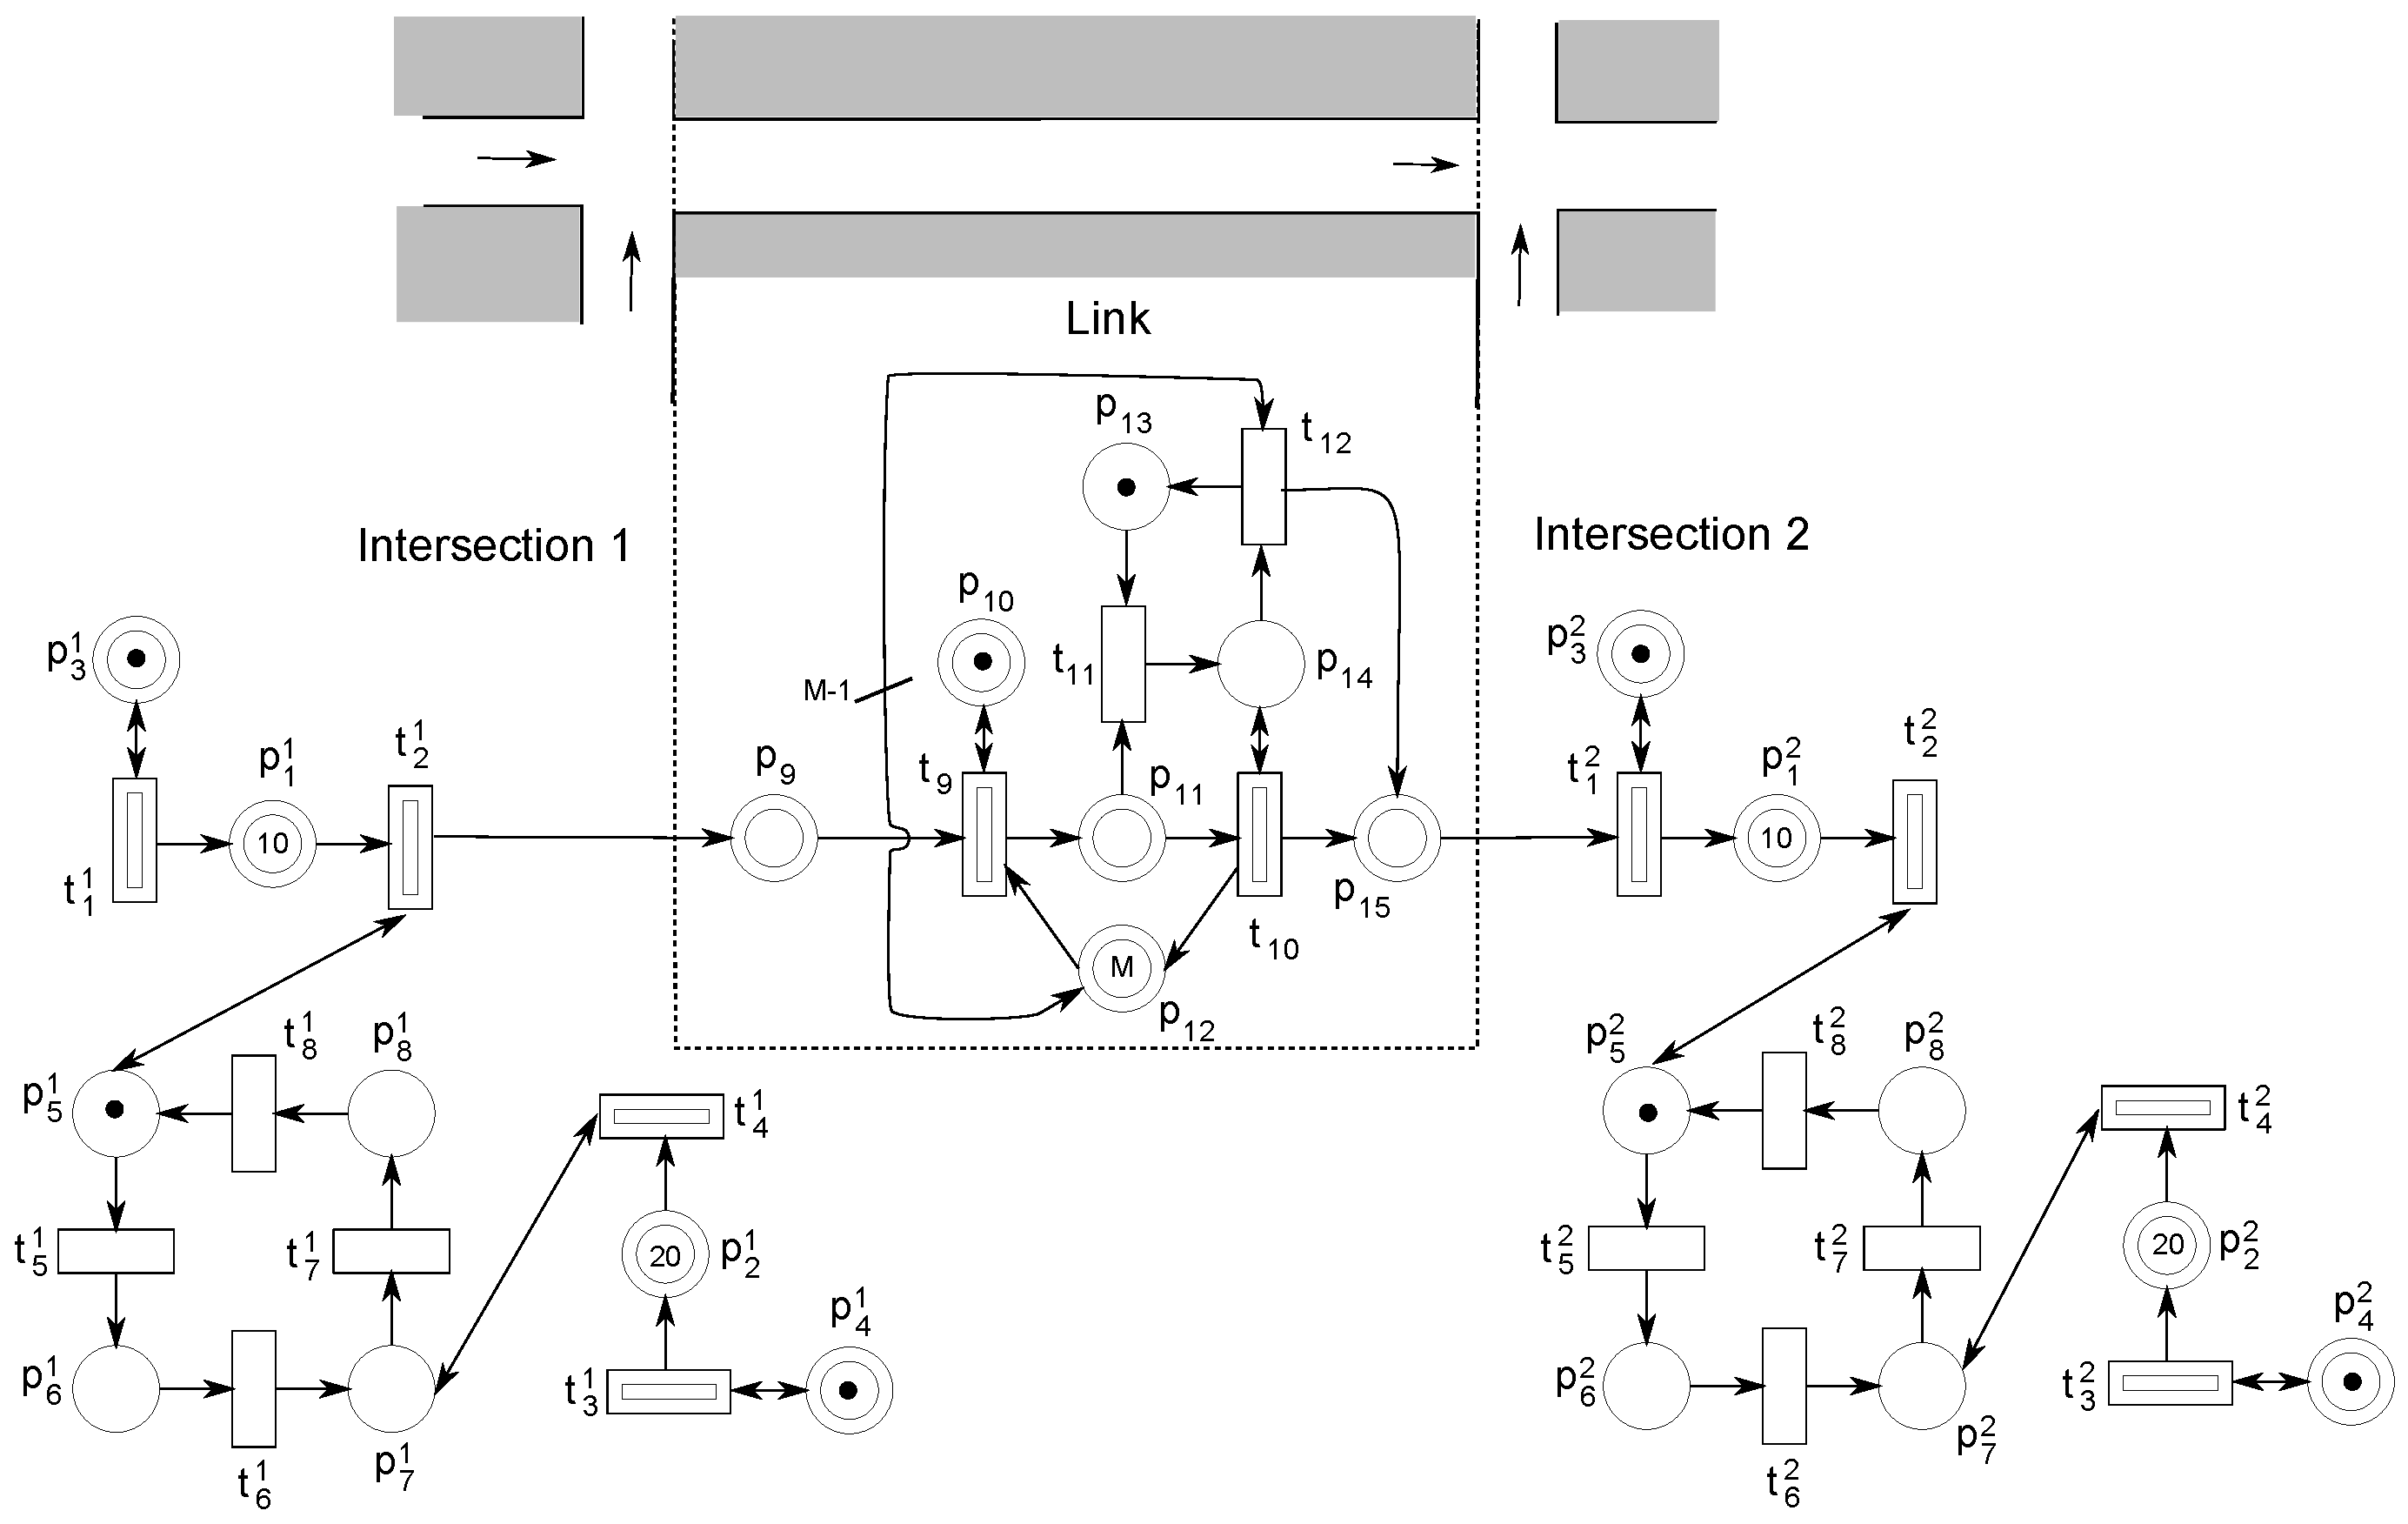
\includegraphics[width=.81\textwidth]{figs/modelo2}
\caption{$HPN$ model of $2$ intersections connected by a link.}
\label{f-traffic}
\end{figure*}


In a HPN, the set of transitions $T$ is partitioned in two sets $T=T^c\cup T^d$,
where $T^c$ contains the set of continuous transitions and $T^d$ the set of discrete
transitions. In contrast to other works, the set of places $P$ is not explicitly
partitioned, i.e., the marking of a place is a natural or real number depending on the
firings of its input and output transitions. Nevertheless, in order to make net models
easier to understand, those places whose marking can be a real non-integer number
will be depicted as double circles (see $p_1^1$ in Fig.~\ref{f-traffic}), and the rest of places will be
depicted as simple circles (such places will have integer markings, see $p_5^1$ in Fig.~\ref{f-traffic}).
Continuous transitions are graphically depicted as two bars (see $t_4^1$ in Fig.~\ref{f-traffic}), while
discrete transitions are represented as empty bars (see $t_5^1$ in Fig.~\ref{f-traffic}), .

Two enabled transitions $t_i$ and $t_j$ are in conflict when they cannot
occur at the same time. For this, it is necessary that $\preset{t_i} \,
\cap \preset{t_j} \neq \emptyset$, and in that case it is said that
$t_i$ and $t_j$ are in structural conflict relation.
%When $\Pre[P,t_i]=\Pre[P,t_j] \neq \zeros$, $t_i$ and $t_j$ are said to be in \emph{equal conflict} relation.
Right and left non negative annullers of the token flow matrix
$\b{C}$ are called T- and P-\emph{semiflows}, respectively.
A semiflow $\vect{v}$ is \emph{minimal} when its
support, $\support{\vect{v}}=\{i\spbar \vect{v}(i)\neq 0\}$, is
not a proper superset of the support of any other semiflow, and
the greatest common divisor of its elements is one.
If there exists $\b{y}>0$ such that $\b{y} \cdot \b{C}=0$,  the net is said to be
\emph{conservative}, and if there exists $\b{x}>0$ satisfying $\b{C}\cdot\b{x}=0$,  the net
is said to be \emph{consistent}. As it will be seen, the basic tasks that
$SimHPN$ can perform on untimed hybrid Petri nets are related to the
computation of minimal T- and P-semiflows.

% Enabling and firing rule
The enabling degree of a continuous transition $t_j \in T$ is:
\begin{equation}
\label{eq:enab}
enab(t_j,\b{m}) = \begin{cases}
 \min \limits_{p_i \in \preset{t_j}}  \left\lfloor\dfrac{m_i}{\Pre(p_i,t_j)}\right\rfloor & \text{ if $t_j \in T^d$}
  \vspace{.2cm}
\\
 \min \limits_{p_i \in \preset{t_j}} \dfrac{m_i}{\Pre(p_i,t_j)} & \text{ if $t_j \in T^c$}
\end{cases}
\end{equation}

Transition $t_j \in T$ is \emph{enabled} at $\b{m}$ iff $enab(t_j,\b{m})>0$.
An enabled transition $t_j \in T$ can fire in any amount $\alpha$ such that
\mbox{$0 \leq \alpha \leq enab(t_j,\b{m})$} and $\alpha\in\nat$ if $t_j \in T^d$
and \mbox{$\alpha\in\rea$} if $t_j \in T^c$. Such a firing leads to a
new marking \mbox{$\b{m'} = \b{m} + \alpha \cdot \C(\cdot,t_j)$}, where $\C = \Post
- \Pre$ is the token-flow matrix and $\C(\cdot,t_j)$ is its $j$ column. If $\b{m}$ is reachable from
$\b{m}_0$ through a finite sequence $\sigma$, the \emph{state (or
fundamental) equation}, $\b{m} =\b{m}_0
+\C \cdot \b{\sigma}$ is satisfied, where $\b{\sigma} \in \rea^{|\mathit{T}|}_{\geq 0}$
is the firing count vector. According to this firing rule the class of nets defined
in Def~\ref{d:uhpn} is equivalent to the class of nets defined in~\cite{BODavid10,ARBaMeGi00}.


\section{Timed Hybrid Petri net  systems}
\label{s:timedHPN}

Different time interpretations can be associated to the firing of transitions.
Once an interpretation is chosen, the state equation can be used to show
the dependency of the marking on time, i.e., $\b{m}(\tau) = \b{m_0} + \C \cdot
\b{\sigma}(\tau)$. The term $\b{\sigma}(\tau)$ is the firing count vector
at time $\tau$. Depending on the chosen time interpretation, the firing
count vector $\sigma_j(\tau)$ of a transition $t_j \in T^c$ is differentiable
with respect to time, and its derivative $f_j(\tau)=\dot{\sigma_j}(\tau)$
represents the \emph{continuous flow} of $t_j$. As for the timing of
discrete transitions, several definitions exist for the flow of continuous
transitions. $SimHPN$ accounts for infinite server and product server semantics
in both continuous and discrete transitions, and additionally, discrete transitions
are also allow to have deterministic delays.

\begin{defn}
\label{d:thpn}
A \emph{Timed Hybrid Petri Net (THPN) system} is a tuple $\langle \N, \b{m}_0, Type, \b{\lambda} \rangle$
where $\langle \N, \b{m}_0\rangle$ is a HPN, $Type:T\rightarrow \{id,pd,dd,ic,pc\}$ establishes the time
semantics of transitions and $\b{\lambda}:T\rightarrow \rea_{\geq 0}$ associates a real parameter to each
transition related to its semantics.
\end{defn}

Any of the following semantics is allowed for a discrete transition $t_i\in T^d$:
\begin{itemize}
\item \emph{Infinite server semantics} ($Type(t_i)=id$): Under infinite server
semantics, the time delay of a transition $t_i$, at a given marking $\b{m}$, is an exponentially distributed
random variable with parameter $\lambda_i\cdot enab(t_i,\b{m})$,
where the integer enabling $enab(t_i,\b{m})$ represents the number of active servers of
$t_i$ at marking $\b{m}$.
\item \emph{Product server semantics} ($Type(t_i)=pd$): Under product server
semantics, the time delay of a transition $t_i$ at $\b{m}$ is an exponentially
distributed random variable with parameter $\lambda_i \cdot
\prod\limits_{p_j\in \preset{t_i}} \left\lfloor\dfrac{\b{m}(p_j)}{\b{Pre}(p_j,t_i)}\right\rfloor$, where
$\prod\limits_{p_j\in \preset{t_i}} \left\lfloor\dfrac{\b{m}(p_j)}{\b{Pre}(p_j,t_i)}\right\rfloor$ is the number of active servers.
\item \emph{Deterministic delay} ($Type(t_i)=dd$): A transition $t_i$ with deterministic
delay is scheduled to fire $1/\lambda_i$ time units after it became enabled.
\end{itemize}

\emph{Conflict resolution:} When several discrete exponential transitions, under either infinite or product server semantics, are in conflict, a racing policy is adopted, i.e., the one with smaller time delay will fire first.

If a discrete transition with deterministic delay is not in conflict with other transitions, it is fired as scheduled, if it is in conflict then
it is fired only if its schedule firing time is less than the firing time of the conflicting
transition. The transition to fire, in the case of several conflicting deterministic transitions
with same scheduled firing instance, is chosen probabilistically assigning the same probability
to each conflicting transition. Furthermore after the firing of a
deterministic transition, the timers of all the transitions in the same conflict are discarded.

For a continuous transition $t_i\in T^c$ the following semantics are allowed:
\begin{itemize}
\item \emph{Infinite server semantics} ($Type(t_i)=ic$): Under \emph{infinite server}
the flow of a transition $t_i$ is:
\begin{equation}\label{eq-flowinf}
f_i=\lambda_i \cdot enab(t_i,\b{m}) = \lambda_i \cdot \min
\limits_{p_j \in \preset{t_i}} \left\{ \frac{m_j}{\b{Pre}(p_j,t_i)}
\right\}
\end{equation}
Such an expression for the flow is obtained from a first order approximation of the
discrete case~\cite{ARSiRe02} and corresponds to the \emph{variable speed} of
(\cite{ARAlDa98})
\item \emph{Product server  semantics} ($Type(t_i)=pc$): In a similar way to discrete
transitions, the continuous flow under product server semantics is given by:
$$f_i=\lambda_i\cdot\prod_{p_j\ \in\ \preset{t_i}}{\biggl\{\frac{m_j}{\b{Pre}(p_j,t_i)}\biggr\}}$$
\end{itemize}

The described supported semantics cover the modeling of a large variety of actions
usually associated to transitions. For instance, infinite server semantics, which are
more general than finite server semantics, are well suited for modeling actions in
manufacturing, transportation and logistic systems~\cite{BODavid10}; product server semantics are
specially useful to modeling population dynamics~\cite{IPSiRe00} and biochemical
reactions~\cite{InHeGiDo08}; and deterministic delays allow one to represent pure
delays and clocks that appear, for instance, when modeling traffic lights in
automotive traffic systems~\cite{IPVaSuBoSi10}.

\newpage
